\documentclass{beamer}
\usetheme{Berlin}
\usepackage{graphicx}
\graphicspath{ {./figures/} }
\usepackage{booktabs}  % beautiful tables
\usepackage{subcaption}
\usepackage[utf8]{inputenc}
\usefonttheme{professionalfonts}
\usepackage{amsmath,amsthm,amssymb,amsfonts}
\usepackage[T1]{fontenc}
\usepackage[sc]{mathpazo}
\usepackage[
backend=biber,
style=alphabetic,
citestyle=authoryear
]{biblatex}
\bibliography{Bib.bib}
% Removes icon in bibliography
\setbeamertemplate{bibliography item}{}

\title{Robust Machine-Learning Approaches for Efficient Functional Dependency Approximation}
\author{Philipp Jung}
\institute[Beuth University of Applied Sciences]
{Beuth University of Applied Sciences\\
\medskip\
philippjung@posteo.de
}
\date{November 27, 2019}

\AtBeginSection[]{
  \begin{frame}
  \vfill
  \centering
  \begin{beamercolorbox}[sep=8pt,center,shadow=true,rounded=true]{title}
    \usebeamerfont{title}\insertsectionhead\par%
  \end{beamercolorbox}
  \vfill
  \end{frame}
}

\begin{document}
\maketitle


\begin{frame}{Overview}
    \tableofcontents
\end{frame}


\section{Motivation}

\begin{frame}
    \frametitle{Example of an FD}
\begin{table}[ht]
    \centering
    \begin{tabular}{rlllr}
        \toprule
        \toprule
        & \multicolumn{3}{c}{left hand side} & \multicolumn{1}{c}{right hand side} \\ \cmidrule(lr{.25em}){1-4} \cmidrule(l{4.75em}){4-5}
        \textsc{Id} & \textsc{First Name} & \textsc{Surname} & \textsc{Zip} & \textsc{Town} \\
        \midrule
        1 & Alice & Smith & 19139 & Munich \\
        2 & Peter& Meyer & 19139 & Munich \\
        3 & Ana & Parker & 19139 & Munich  \\
        4 & John & Pick & 12055 & Berlin \\
        5 & John & Pick & 19139 & Munich \\
        \bottomrule
        \bottomrule
    \end{tabular}
    \caption{Example of the non-minimal FD $\textsc{\{Id, First Name, Surname, Zip\}}~\rightarrow~\textsc{Town}$.}
\end{table}
\end{frame}

\begin{frame}
    \frametitle{FD Fields of Application}
    FDs are constraints on a relational scheme commonly used for
    \begin{itemize}
        \item schema normalization of relational databases
        \item data cleaning, e.g. HoloClean\footcite{HEI19}
        \item data exploration
    \end{itemize}
\end{frame}

\begin{frame}
    \frametitle{Challenges of FD Detection}
    \begin{block}{Remark}
        FD detection is a particularly complex problem to solve.
    \end{block}
\end{frame}

\begin{frame}
    \frametitle{FD Detection Search Space Size}
    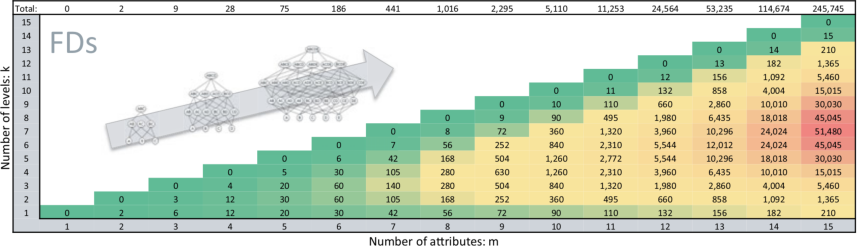
\includegraphics[width=\textwidth]{fd_detection_complexity}\footnotetext{Image from~\cite{ABE19}}
    \newline
    \vspace*{0.3 cm}
    \newline
    The number of FD candidates for $m$ attributes is $\mathcal{O}(\frac{m}{2} \cdot 2^m)$.
\end{frame}

\begin{frame}
    \frametitle{Learned Algorithms}
    Kraska et al.\ showed in 2018 that a Binary Tree can be interpreted
    as a learned index structure.\footcite{KRA18}
\end{frame}

\begin{frame}
    \frametitle{BTree as a Learned Model}
    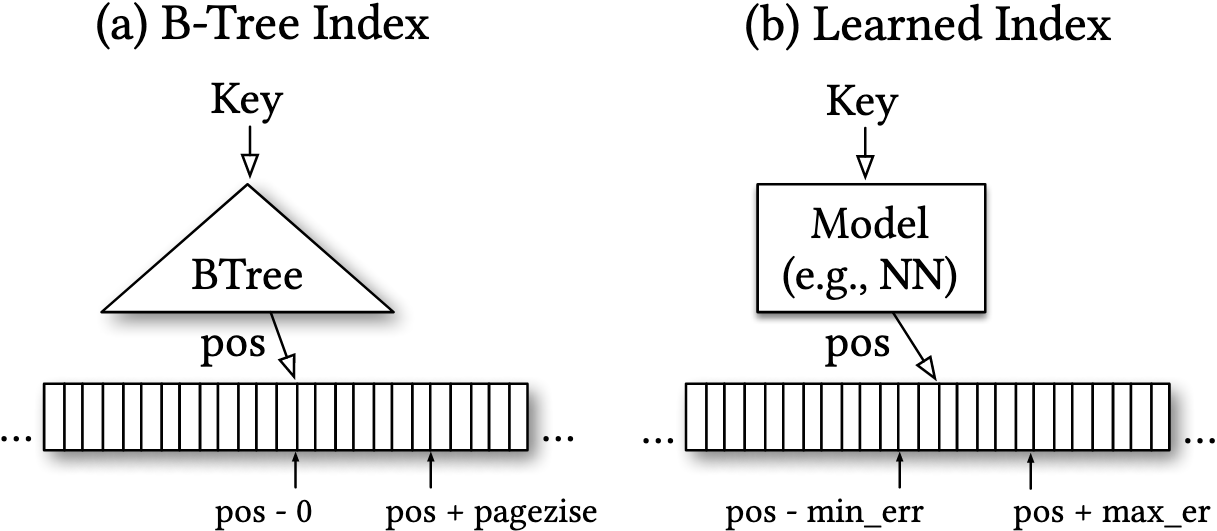
\includegraphics[width=\textwidth]{btree_as_model}
    \footnotetext{Image from~\cite{KRA18}}
\end{frame}

\begin{frame}
    \frametitle{Learning FDs}
    \begin{block}{Remark}
        Learned algorithms offer a new research-directory when solving old algorithmic problems.
    \end{block}
\end{frame}

\section{Objectives}
\begin{frame}
    \frametitle{Research Objectives}
    \begin{itemize}
        \item Interpret FDs as \emph{learned} constraints
        \item Train data imputation models with DataWig and benchmark them against FD-based models
        \item Identify similarities and leverage them to derive FDs from learned models
        \item Detect minimal FDs
    \end{itemize}
\end{frame}

\begin{frame}
    \frametitle{DataWig}
    \begin{itemize}
        \item DataWig is a framework for learning models to impute missing values in tables
        \item Data imputation: Replace missing or faulty data
        \item Models trained by DataWig use either regression or multi-label classification
        \item DataWig models can be benchmarked against FD Imputer
    \end{itemize}
\end{frame}

\section{FD Imputer}
\begin{frame}
    \frametitle{FD Imputer: FDs as Models}
    \begin{itemize}
        \item Interpret FDs as rules for data imputation
        \item Write FD Imputer: An imputation model entirely based on FDs
        \item Measure \emph{Robustness}: Either the F1-Score or the MSE that FD Imputer obtains for a FD
    \end{itemize}
\end{frame}

\begin{frame}
    \frametitle{How FD Imputer works}
    \begin{enumerate}
        \item Split dataset in train-set and test-set
        \item Detect FDs on train-set using HyFD\footcite{PAP16}
        \item For each FD, impute the right hand side for each row in the \textbf{test}-set. Do so by finding a tuple with equal left hand side in the \textbf{train}-set
        \item Compute \emph{Robustness} by evaluating FD Imputer's performance for each FD (F1-Score or Mean Squared Error)
    \end{enumerate}
\end{frame}

\begin{frame}
    \frametitle{FD Imputer Functionality Example}
\begin{table}[ht]
    \begin{subtable}[c]{0.9\textwidth}
        \centering
        \begin{tabular}{llll}
            \textsc{A} & \textsc{B} & \textsc{C} & \textsc{D}  \\
        \toprule
        \toprule
            Green & Bus & Portugal & Lisbon \\
            Yellow & Car & Portugal & Lisbon \\
        \bottomrule
        \bottomrule
        \end{tabular}
        \subcaption{Train set}
    \end{subtable}
    \newline
    \vspace*{0.3 cm}
    \newline
\begin{subtable}[c]{0.9\textwidth}
        \centering
        \begin{tabular}{llll}
        \textsc{A} & \textsc{B} & \textsc{C} & \textsc{D} \\
        \toprule
        \toprule
        Yellow & Bus & Spain & ? \\
        Blue & Bus & Portugal & ? \\
        \bottomrule
        \bottomrule
        \end{tabular}
        \subcaption{Test set}
    \end{subtable}
\end{table}
In this example, FD Imputer uses the FD \textsc{C}~$\rightarrow$~\textsc{D}.
\end{frame}

\begin{frame}
    \frametitle{FD Imputer Functionality Example}
\begin{table}[ht]
    \begin{subtable}[c]{0.9\textwidth}
        \centering
        \begin{tabular}{llll}
            \textsc{A} & \textsc{B} & \textsc{C} & \textsc{D}  \\
        \toprule
        \toprule
            Green & Bus & Portugal & Lisbon \\
            Yellow & Car & Portugal & Lisbon \\
        \bottomrule
        \bottomrule
        \end{tabular}
        \subcaption{Train set}
    \end{subtable}
    \newline
    \vspace*{0.3 cm}
    \newline
\begin{subtable}[c]{0.9\textwidth}
        \centering
        \begin{tabular}{llll}
        \textsc{A} & \textsc{B} & \textsc{C} & \textsc{D} \\
        \toprule
        \toprule
        Yellow & Bus & Spain & - \\
        Blue & Bus & Portugal & Lisbon \\
        \bottomrule
        \bottomrule
        \end{tabular}
        \subcaption{Test set}
    \end{subtable}
\end{table}
In this example, FD Imputer uses the FD \textsc{C}~$\rightarrow$~\textsc{D}.
\end{frame}

\begin{frame}
    \frametitle{Benchmarking FD Imputer}
    \begin{table}[ht]
        \centering
        \begin{tabular}{lrrrrrr}
            \toprule
            \toprule
            Dataset & \#FDs\textsubscript{train} & \#FD (F1 = 0) & F1\textsubscript{mean} & F1\textsubscript{max} \\
            \midrule
            Abalone & 193 & 45 & 0.0008 & 0.0048 \\
            Adult & 88 & 10 & 0.0669 & 1.0000 \\
            Balance S. & 7 & 6 & 0.0000 & 0.0000 \\
            Breast C. W. & 77 & 10 & 0.2198 & 0.7539 \\
            Chess & 9 & 8 & 0.0000 & 0.0000 \\
            Iris & 8 & 1 & 0.1274 & 0.2252 \\
            Letter & 80 & 17 & 0.2347 & 0.3737 \\
            Nursery & 11 & 10 & 0.0000 & 0.0000  \\
            \bottomrule
            \bottomrule
        \end{tabular}
        \caption{Performance of the FD Imputer on a selection of UCI datasets.}\label{tab:fd-imputer-performance}
    \end{table}
\end{frame}

\begin{frame}
    \frametitle{Benchmarking FD Imputer: Ranking for Robustness}
    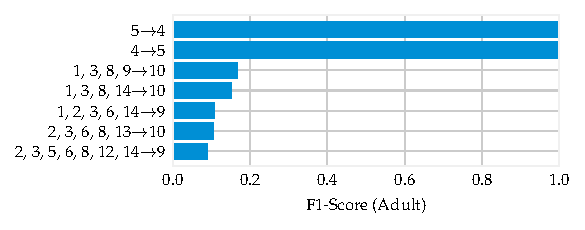
\includegraphics[width=\textwidth]{f1_fd_imputer.pdf}
\end{frame}

\begin{frame}
    \frametitle{Benchmarking FD Imputer: Comparison with DataWig Model}
    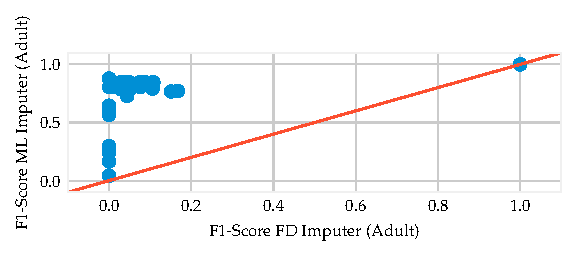
\includegraphics[width=\textwidth]{f1_ml_fd.pdf}
\end{frame}

\begin{frame}
    \frametitle{Summary of FD Imputer Results}
    \begin{itemize}
        \item Some FDs are more robust than others
        \item FD Imputer performs generally worse than the model trained with DataWig
        \item This concerns only classifiable data -- it is generally impossible to impute continuous numerical data with FD Imputer
    \end{itemize}
\end{frame}

\begin{frame}
    \frametitle{FD Imputer is Overfitting by Design}
    \begin{block}{Haykin 2008}
        ``[Overfitting] is essentially a `look-up table', which implies that the input-output mapping [\dots] is not smooth.''\footcite[p.~165]{HAY08}
    \end{block}
    \pause
    \begin{itemize}
        \item Due to the implementation of FD Imputer, the train-set is merely a table to look up imputation values
        \item No generalization takes place whatsoever
        \item No empirical risk minimization (ERM) is applied!
    \end{itemize}
\end{frame}

\begin{frame}
    \frametitle{Deriving FDs from Trained Models}
    \begin{itemize}
        \item When overfitting DataWig models, one cannot control that overfitting takes place on LHS FD-attributes
    \end{itemize}
    \begin{block}{Proposition}
        In consequence, it does not appear to be possible to derive FDs with ERM-based imputation models.
    \end{block}
\end{frame}

\begin{frame}
    \frametitle{Deriving FDs from Trained Models}
    But what about Relaxed Functional Dependencies (RFDs)?
\end{frame}
\section{DepDetector}
\begin{frame}
    \frametitle{RFDs as Models}
    \begin{itemize}
        \item An RFD is based on the definition of an FD
        \item It alters that definition to serve a specific purpose
        \item There are many RFDs defined, such as Metric Functional Dependencies, Conditional Functional Dependencies or Approximate Functional Dependencies.
    \end{itemize}
\end{frame}

\begin{frame}
    \frametitle{Example of an RFD}
    \begin{Example}
        Koudas et al.\ introduce Metric Functional Dependencies (MFDs) to find constraints on tables that contain rows with slightly different formatting or slightly deviating values.\footcite{KOU09}
    \end{Example}
\end{frame}

\begin{frame}
    \frametitle{Example for Noisy Data}
    \begin{table}[ht]
        \centering
        \begin{tabular}{lcccc}
            \toprule
            \toprule
            \textsc{Id} & First name & Last name & \textsc{Zip} & Town \\
            \midrule
            1 & Alice & Smith & 19139 & Munich \\
            \textbf{2} & \textbf{Peter}& \textbf{Meyer} & \textbf{19139} & \textbf{Muinch} \\
            3 & Ana & Parker & 19139 & Munich \\
            4 & John & Pick & 12055 & Berlin \\
            \bottomrule
            \bottomrule
        \end{tabular}
    \end{table}
The FD \textsc{Zip}~$\rightarrow$~\textsc{Town} is violated by the second row. A MFD that considers the Levenshtein distance between two entries rather than exact equality can still detect the constraint.
\end{frame}

\begin{frame}
    \frametitle{RFDs as Models}
    \begin{itemize}
        \item Due to their their training being ERM-based, DataWig models are capable of learning constraints on noisy data as well
        \item During training, DataWig models ``learn'' relaxations -- there is no need to manually set up a threshold of a Levenshtein distance as in the previous example
    \end{itemize}
    \pause
    \begin{block}{Question}
        How does one find a \emph{minimal} dependency with this approach?
    \end{block}
\end{frame}

\begin{frame}
    \frametitle{Functionality of DepDetector}
    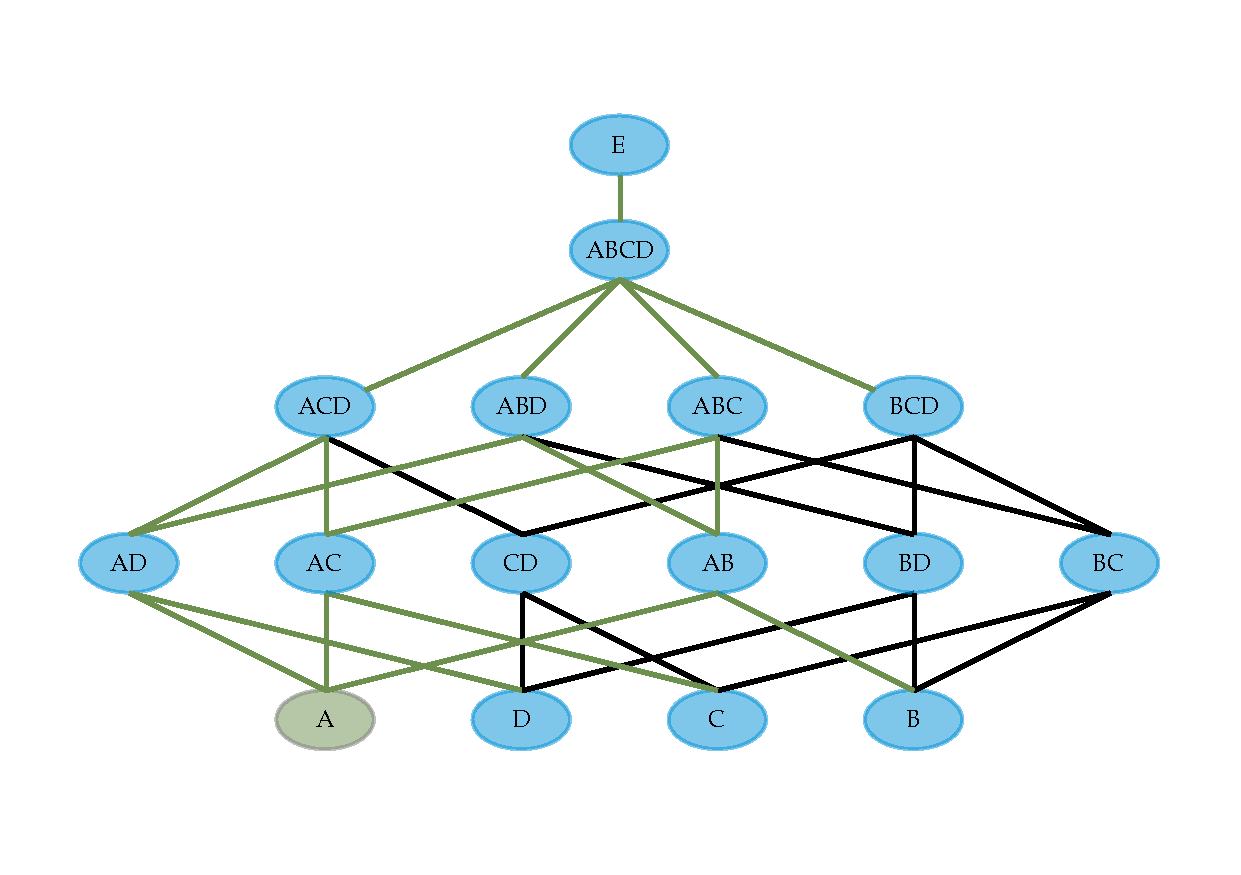
\includegraphics[width=.95\textwidth]{search-tree-fd.pdf}
\end{frame}

\begin{frame}
    \frametitle{Functionality of DepDetector}
    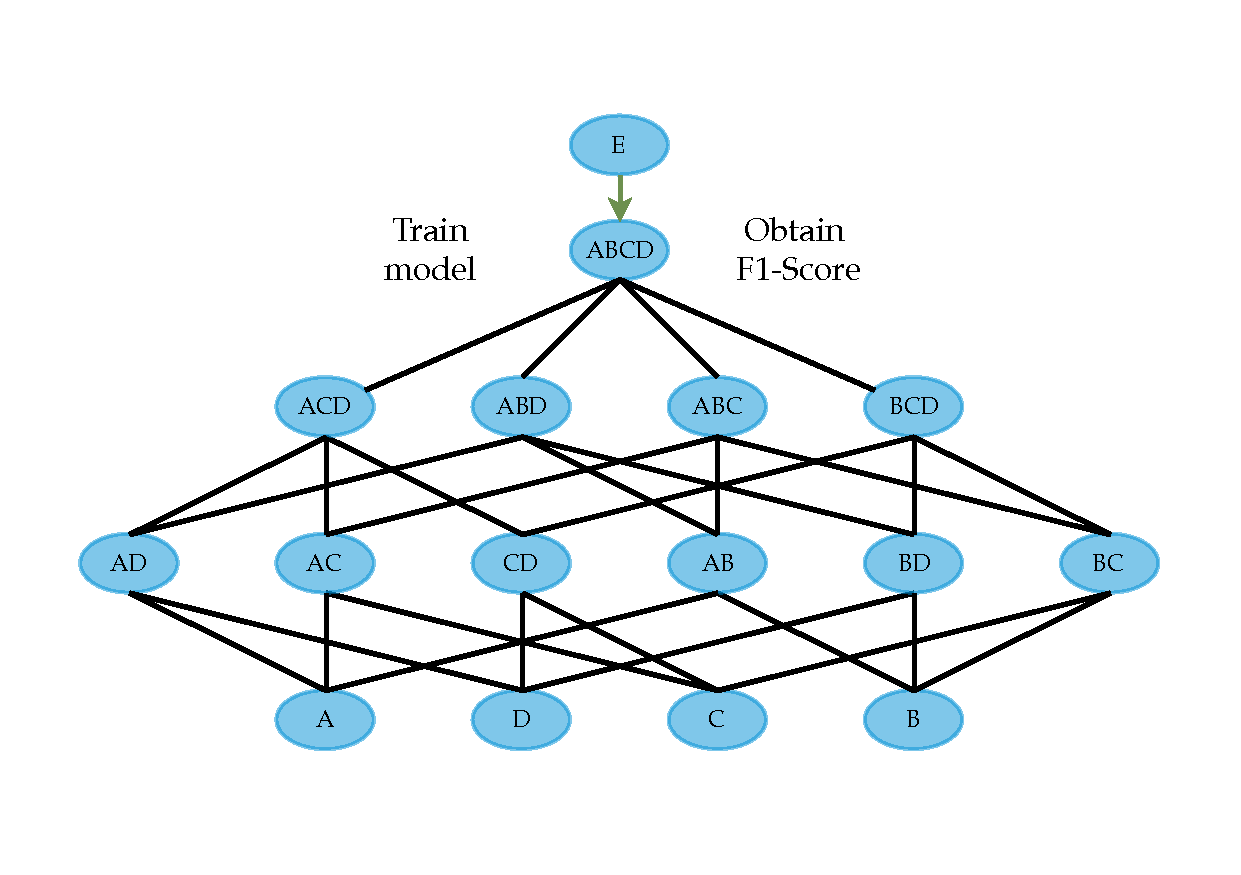
\includegraphics[width=.95\textwidth]{min-dep-step-1.pdf}
\end{frame}

\begin{frame}
    \frametitle{Functionality of DepDetector}
    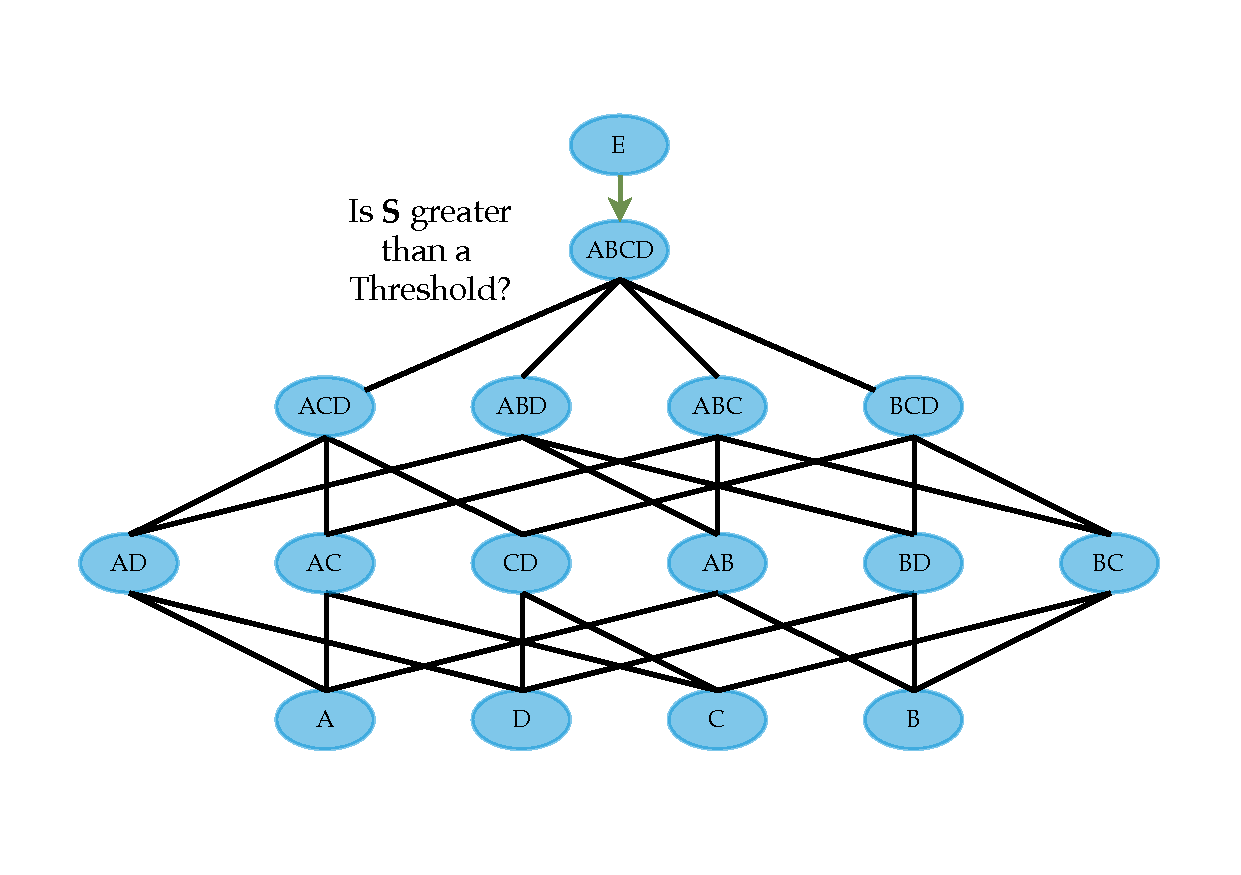
\includegraphics[width=.95\textwidth]{min-dep-step-2.pdf}
\end{frame}

\begin{frame}
    \frametitle{Functionality of DepDetector}
    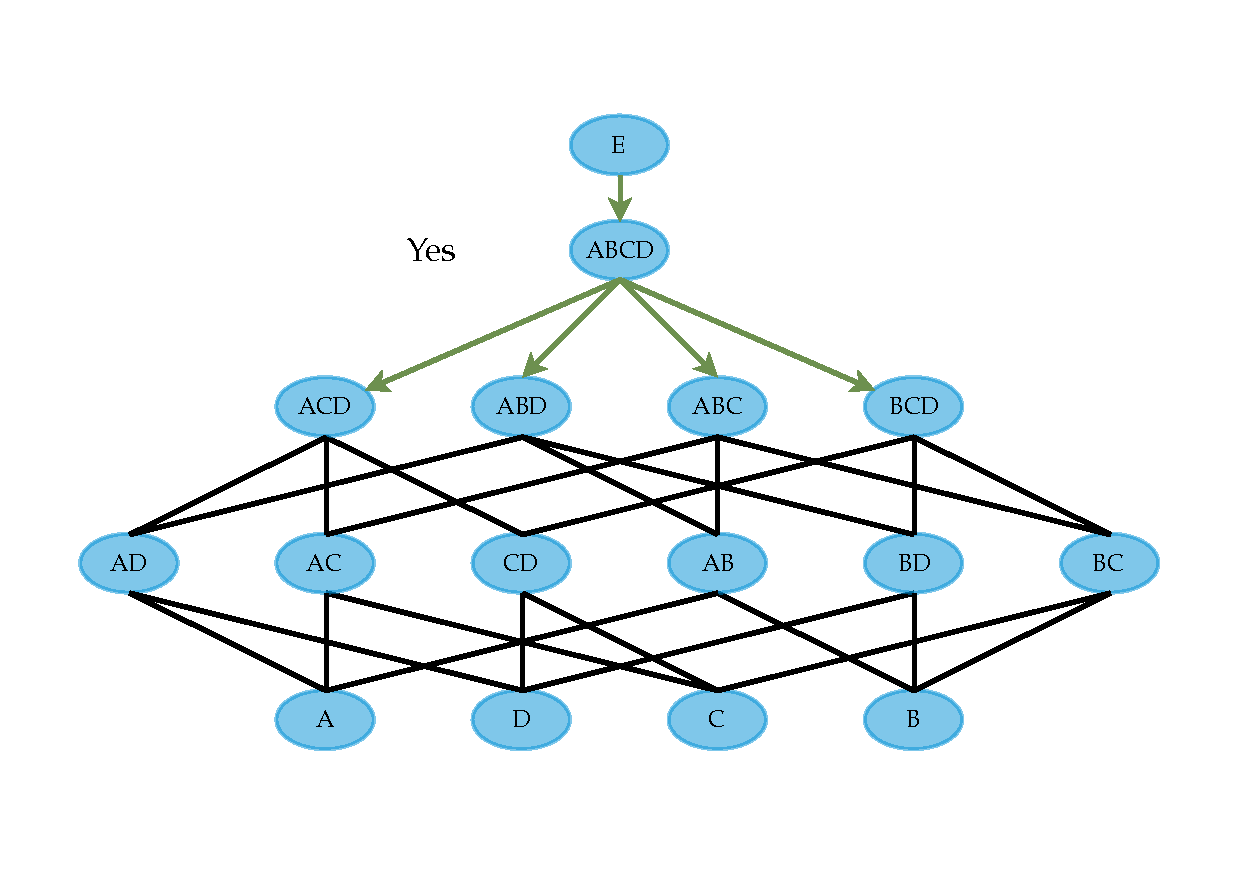
\includegraphics[width=.95\textwidth]{min-dep-step-3.pdf}
\end{frame}

\begin{frame}
    \frametitle{Functionality of DepDetector}
    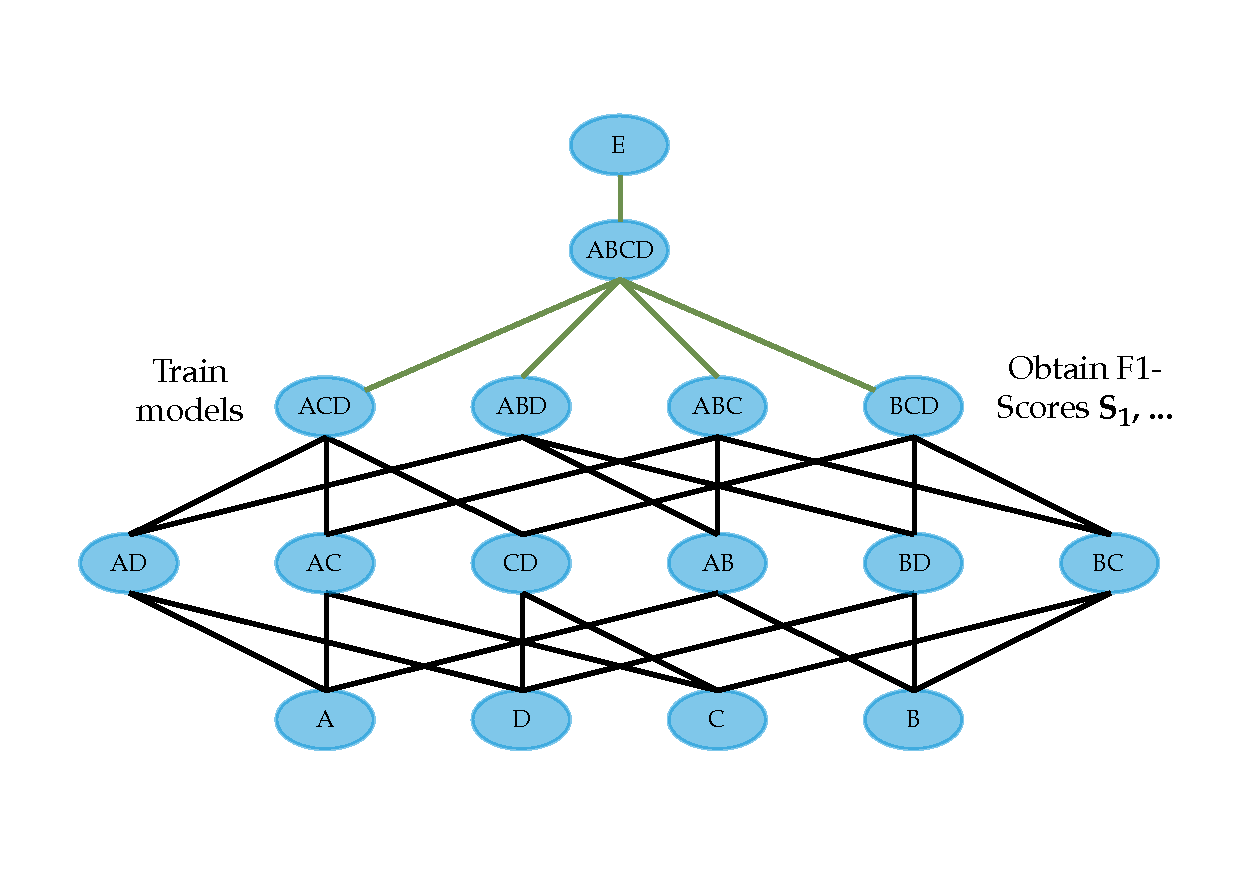
\includegraphics[width=.95\textwidth]{min-dep-step-4.pdf}
\end{frame}

\begin{frame}
    \frametitle{Functionality of DepDetector}
    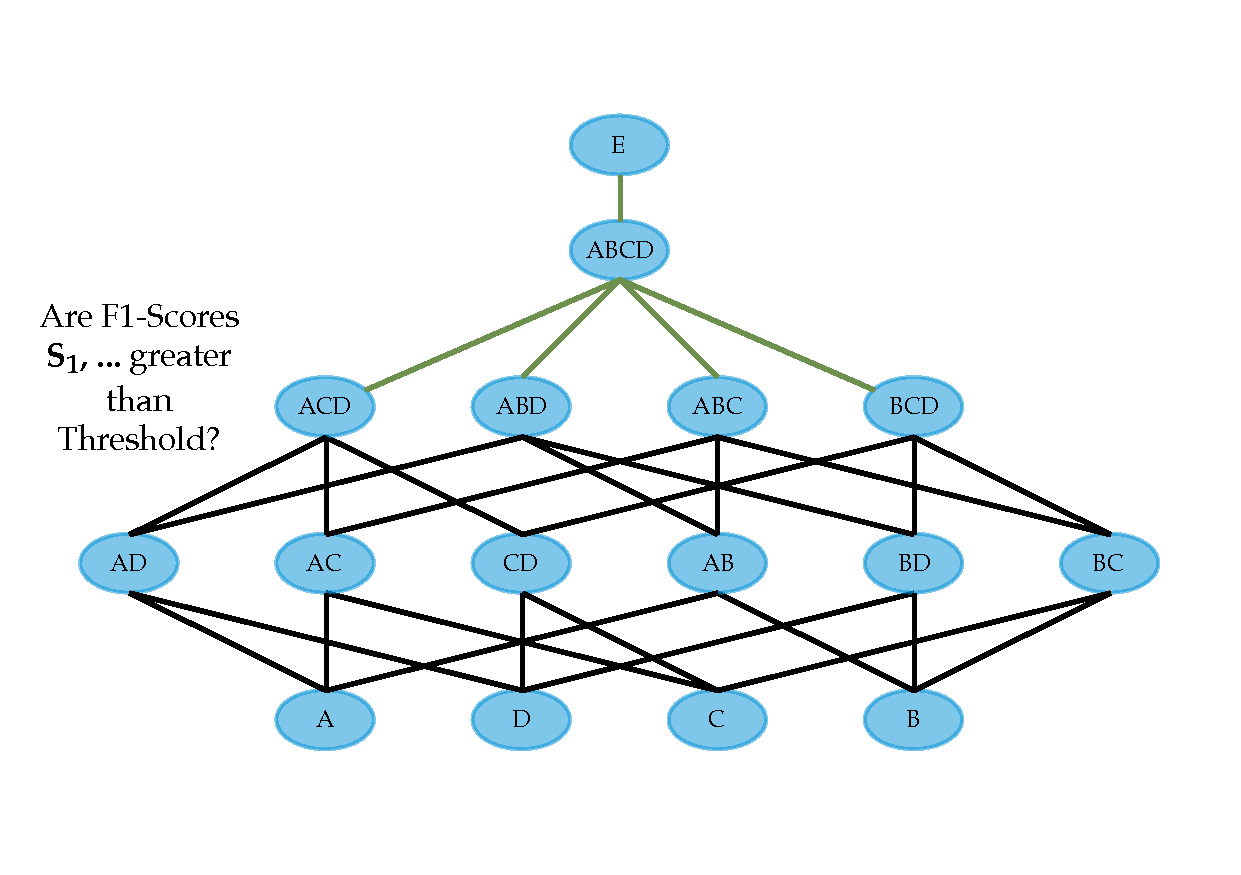
\includegraphics[width=.95\textwidth]{min-dep-step-5.pdf}
\end{frame}

\begin{frame}
    \frametitle{Functionality of DepDetector}
    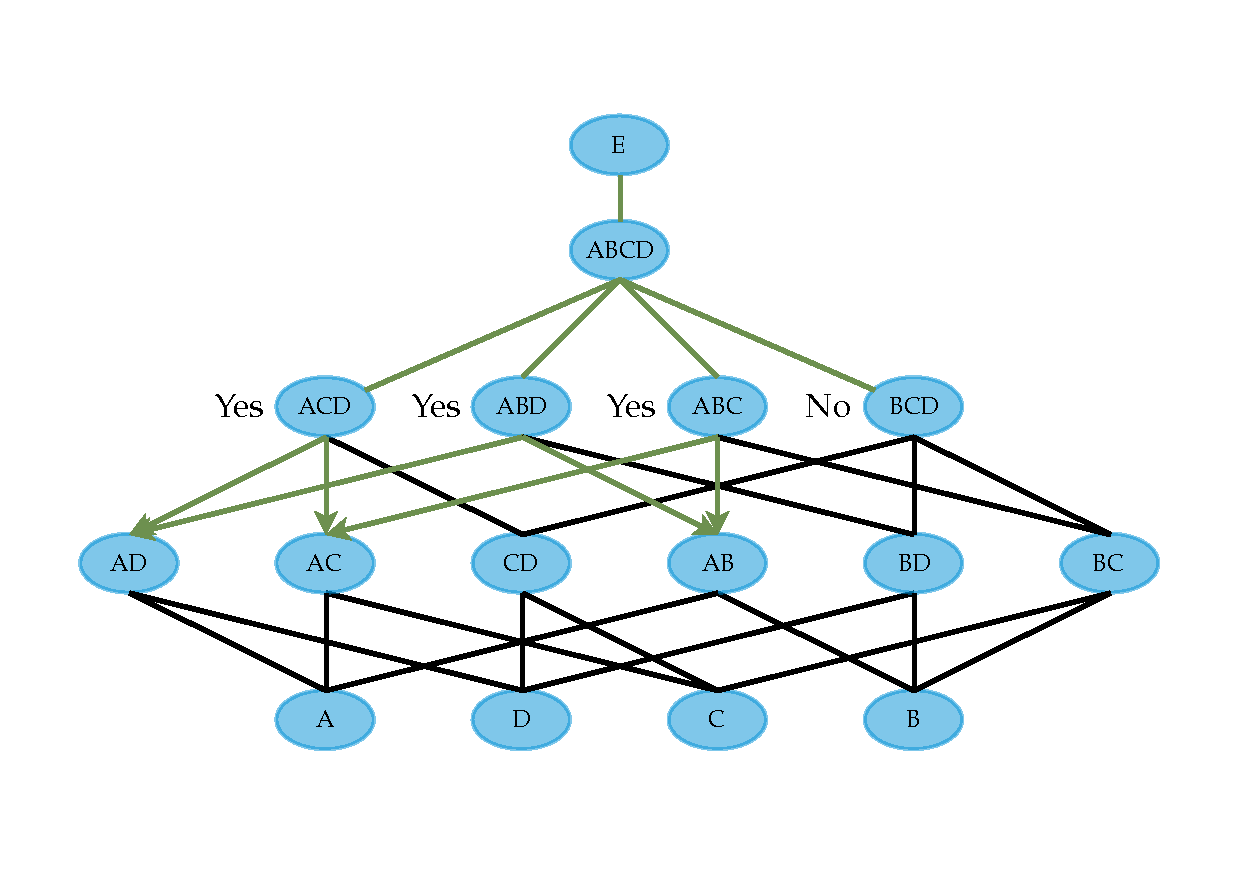
\includegraphics[width=.95\textwidth]{min-dep-step-6.pdf}
\end{frame}

\begin{frame}
    \frametitle{Functionality of DepDetector}
    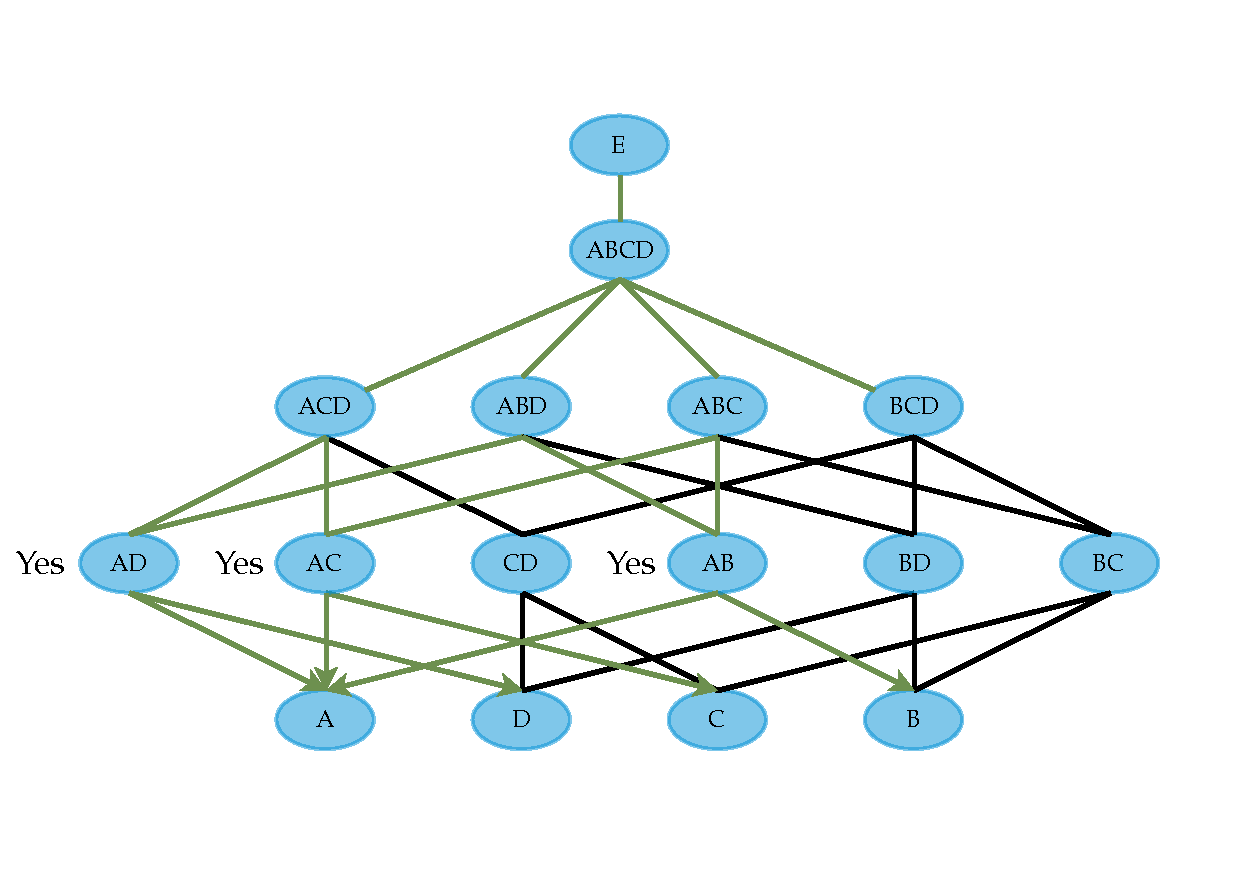
\includegraphics[width=.95\textwidth]{min-dep-step-7.pdf}
\end{frame}

\begin{frame}
    \frametitle{Functionality of DepDetector}
    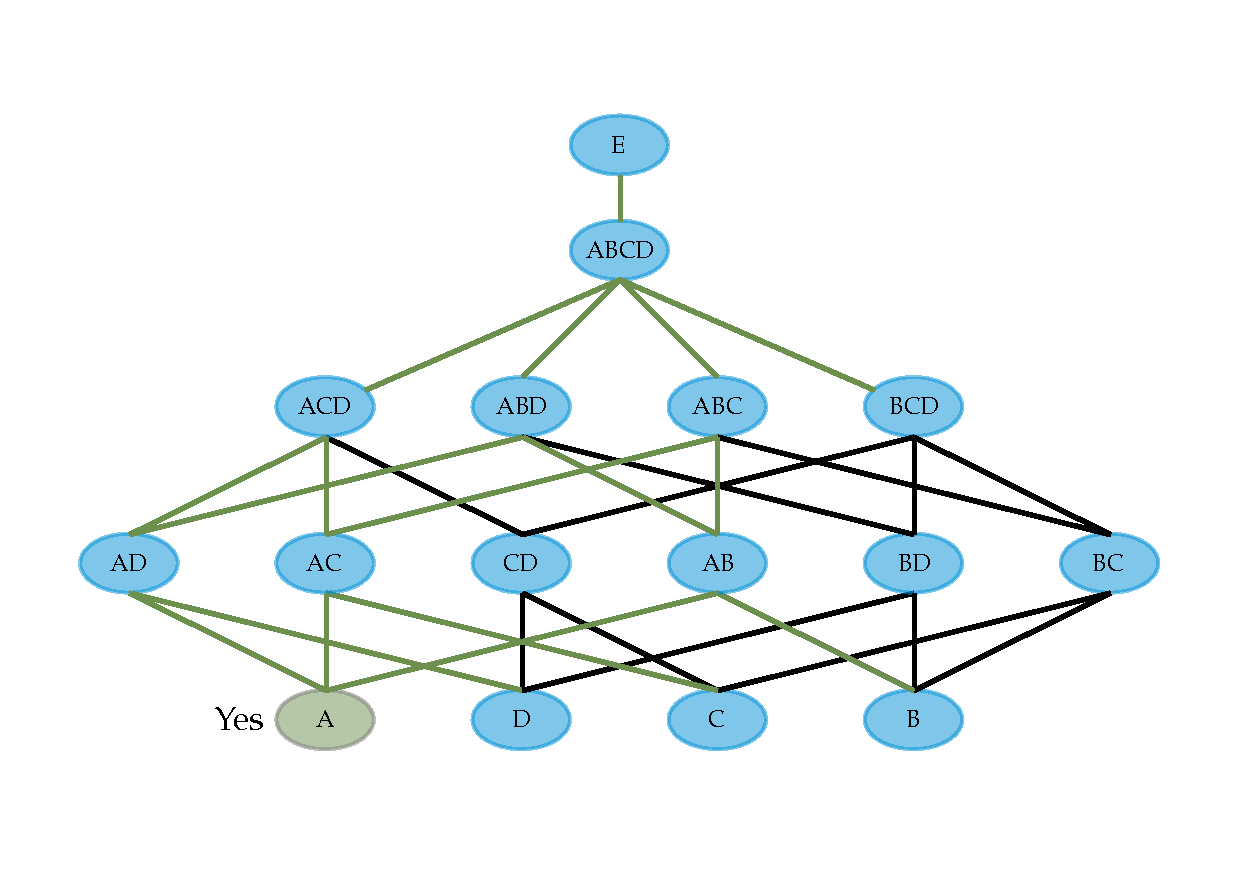
\includegraphics[width=.95\textwidth]{min-dep-step-8.pdf}
\end{frame}

\begin{frame}
    \frametitle{DepDetector Properties}
    \begin{itemize}
        \item DepDetector solves an optimization problem on a directed graph
        \item DepDetector depends on one threshold for classifiable data and one threshold for continous numerical data
    \end{itemize}
\end{frame}

\begin{frame}
    \frametitle{DepDetector Properties}
    \begin{block}{Proposition}
        Machine learning classifier/regressor models may have the potential to unify a number of RFDs.
    \end{block}
\end{frame}

\begin{frame}
    \frametitle{Summary of DepDetector Results}
    \begin{table}[ht]
        \centering
        \begin{tabular}{lrrrrrr}
            \toprule
            \toprule
            & & & & \multicolumn{1}{c}{Greedy} & \multicolumn{1}{c}{Complete} \\
            Dataset & Cols & Rows & \# FDs & dependencies & dependencies \\
            \midrule
            Abalone & 10 & 4177 & 175 & 7~(42~min) & TL \\
            Adult & 16 & 32561 & 93 & TL & TL \\
            Balance-S. & 6 & 625 & 7 & 3~(67~s) & 3~(80~s) \\
            Chess & 8 & 28056 & 9 & 1~(117~min) & 1~(340~min) \\
            Iris & 6 & 150 & 9 & 5~(38~s) & 8~(43s) \\
            Letter & 18 & 20000 & 78 & TL & TL \\
            Nursery & 11 & 12960 & 11 & 3~(110~min) & TL \\
            \bottomrule
            \bottomrule
        \end{tabular}
    \end{table}
`TL' indicates a time limit of 350~min.
\end{frame}

\section{Prospects}
\begin{frame}
    \frametitle{Prospects for further Research}
    \begin{itemize}
        \item Minimal dependency detection algorithms for learned relaxations can be further optimized (Concurrency, applying Graph-Theory)
        \item A complexity analysis for DepDetector can be performed
        \item Approaches to calculate thresholds from the data can be introduced
    \end{itemize}
\end{frame}

\begin{frame}
    \begin{block}{}
        Thank you for your attention!
    \end{block}
\end{frame}
\begin{frame}[allowframebreaks]
\frametitle{References}
\printbibliography
\end{frame}

\section*{Additional Slides}
\begin{frame}
    \frametitle{Benchmarking FD Imputer Continuous Data}
    \begin{table}[ht]
        \centering
        \begin{tabular}{lrrr}
            \toprule
            \toprule
            Dataset & \# cFDs\textsubscript{train} & \# 0-Coverage cFDs  & Coverage (\%) \\
            \midrule
            Abalone & 139 & 84 & 0.1277 \\
            Adult & 11 & 5 & 0.1217 \\
            Balance S. & 1 & 1 & 0.0000 \\
            Breast C. W. & 1 & 1 & 0.0000 \\
            Chess & 1 & 1 & 0.0000 \\
            Iris & 4 & 4 & 0.0000 \\
            Letter & 0 & 0 & - \\
            Nursery & 1 & 1 & 0.0000 \\
            \bottomrule
            \bottomrule
        \end{tabular}
        \caption{Imputation coverage of FD Imputer on all UCI datasets for which FDs with continuous data in the RHS were detected.}\label{tab:fd-imputer-mse}
    \end{table}
\end{frame}

\begin{frame}
    \frametitle{FD Imputer Continuous Data Definitions}
    \begin{align*}
        \text{mean missing values per cFD} = \sum_{i} \frac{\text{missing imputations}}{\text{cFD}_i} \cdot \left(\text{\# cFDs}\right)^{-1} \\
        \text{mean coverage} = \left( 1 - \frac{\text{mean missing values per cFD}}{\text{\# rows in }r_{test}} \right) \cdot 100
    \end{align*}

\end{frame}

\begin{frame}
    \frametitle{Machine Learning Models}
    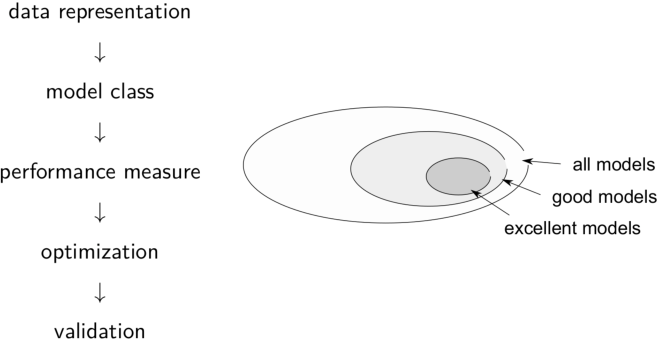
\includegraphics[width=.95\textwidth]{mi-models.pdf}
    \footnotetext{Image from Prof.\ Obermeyer, Neural Information Processing Group TU Berlin}
\end{frame}

\begin{frame}
    \frametitle{Definition Robustness Continous Data}
If \textsc{A} contains continuous numerical data, the MSE is determined to measure robustness:
\begin{align}\label{eq:robustness-mse}
    \text{robustness\textsubscript{MSE}} = \frac{1}{p-m}\sum_{i=m+1}^{p} \left(t_{i}^{\ast}[A] - t_{i}^{\prime}[A]\right)^2.
\end{align}
Here, \( p \in \mathbb{N} \) denotes the number of tuples in a relational instance and \( m \) is the number of imputed tuples.
\end{frame}

\begin{frame}
    \frametitle{Definition Robustness Classifiable Data}
    If \textsc{A} contains classifiable data, the F1-Score is calculated to measure robustness:
    \begin{align}\label{eq:robustness-f1-score}
        \text{robustness\textsubscript{F1-Score}} = {\left(\frac{Recall(r_{imp}, r_{test})^{-1} + Precision(r_{imp}, r_{test})^{-1}}{2}\right)}^{-1}
    \end{align}
\end{frame}

\begin{frame}
    \frametitle{Empirical Risk Minimization}
    \begin{itemize}
        \item We cannot know how an algorithm will be influenced when it is used in practice (\emph{risk})
        \item We thus simulate the fact that the true distribution of data is unknown by creating models on a subset of the whole dataset (\emph{empirical risk})
        \item By minimizing the empirical risk and preventing overfitting by cross-validation or train/test validation, we make models resistant towards noise
    \end{itemize}
\end{frame}

\begin{frame}
    \frametitle{ERM and Overfitting}
    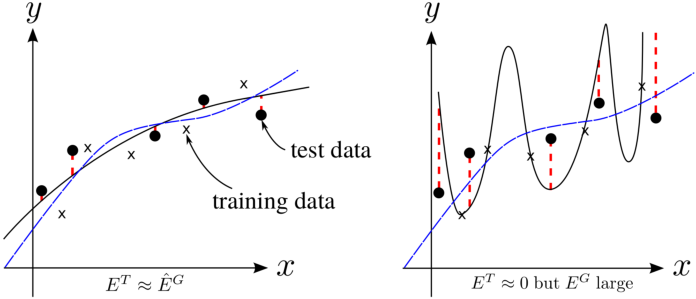
\includegraphics[width=\textwidth]{erm-overfitting}
\end{frame}

\end{document}
